\chapter{Double Beta Decay}
\label{chap:Beta Decay}

While a lepton-violating process such as that in \autoref{fig:0nuBB} would an incredible result to discover in the laboratory, it's not quite so simple as to obtain a soup of down quarks and wait for them to decay into up quarks and electrons or to look at the time-reversed process and use electron beams to produce up and down quarks! The way that an interaction such as the one shown \autoref{fig:0nuBB} could feasibly be discovered in a laboratory setting is through decays of nuclei, namely through neutrinoless double-beta decay. 

\section{Beta Decay}
\label{sec:Beta Decay}
Beta decay is a well-known process that occurs in many nuclei as the mechanism by which nuclei can change their number of protons, Z, while keeping the number of total nucleons, A, constant in the decays
\begin{align}
    (Z, A) & \rightarrow (Z+1, A)+\textrm{e}+\Bar{\nu}_e \label{eq:neutrondecay} \\
    (Z, A) & \rightarrow (Z-1, A)+\Bar{\textrm{e}}+\nu_e \label{eq:protondecay} 
\end{align}

\begin{figure}[tbph]
    \centering
    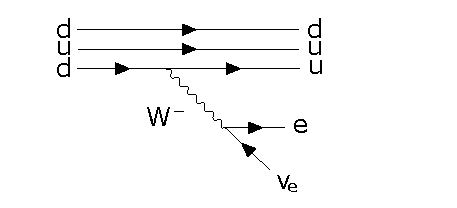
\includegraphics[width=0.8\linewidth]{Figures/NeutronBetaDecay.pdf}
    \caption[Beta Decay Feynman diagram for a neutron converting to a proton]{The Feynman diagram for beta decay for a neutron to convert to a proton inside a nucleus by emitting an electron and and anti-neutrino.}
    \label{fig:NeutronBetaDecay}
    
\end{figure}

The process in \autoref{eq:neutrondecay} is shown in \autoref{fig:NeutronBetaDecay}, and the accompanying process, \autoref{eq:protondecay}, while kinematically forbidden in free protons because they are lighter than neutrons, is able to occur in nuclei where the change in binding energies of the resultant nucleus is able to compensate for the proton and neutron mass difference.

\subsection{History of Beta Decay}
Historically, the discovery and physics advancements from double beta decay can shed some light on the current state of the field of neutrinoless double-beta decay searches. In particular, when the energy spectrum of beta decays were first discovered, it took the community by surprise that the spectrum was continuous and not peaked at a single value as, e.g., an alpha decay would be \cite{o.vonbayero.hahnl.meitner}. This seemed to suggest that either energy was not conserved in the interaction or that there was another seemingly massless undetected particle that was escaping the interaction and taking away energy. To resolve this issue, Wolfgang Pauli speculated in a famous letter in 1930 to ``dear radioactive ladies and gentlemen" about the existence of the neutrino particle to account for the missing energy \cite{pauli_1930}. The physics community at the time was quite skeptical of such a theory, as it posited a particle seemingly impossible to detect in order to conserve energy, and Enrico Fermi was even rejected on these grounds from publishing his theory on beta decay in the journal Nature \cite{fermi_1934}. Luckily, neutrinos are not impossible to detect and were first discovered in the Cowan-Reines experiment only 20 years later in 1954 \cite{PhysRev.92.830}. Using beta capture, a similar process to beta decay, this experiment observed antineutrinos interacting with ``free" protons in hydrogens atoms in a water tank. In this way, beta decay has been used to observe new physics and has been both an active and fruitful area of research since it was first observed. Even recently, observations of neutrinos have resulted in the discovery of neutrino oscillations, discussed in \autoref{ssec:NeutrinoMassesandOscillation}, which was the first confirmation of physics beyond the Standard Model.

\section{Double-Beta Decay}
\label{sec:Double Beta Decay}
Since beta decay is an allowed process, a decay in which two decays happen simultaneously, double-beta decay, should also be allowed. However, for most nuclei, this second-order weak process is dwarfed by the significantly higher rates of single-beta decay. For example, beta decays have a typical half-life on the order of $10^9~\textrm{yr}$, e.g. K-40 decays with a half-life of $1.251\times10^{9}~\textrm{yr}$, while typical half-lives for double-beta decay are on the order of $10^{20}~\textrm{yr}$. This many orders of magnitude higher rate makes measuring double-beta decay virtually impossible as the single-beta decay rate would be an insurmountable background. However, the exception to this occurs in some even-even nuclei wherein single beta decay is energetically forbidden, but double beta decay is allowed, shown in \autoref{fig:parabola_odd} and \autoref{fig:parabola_even}. Of the 35 naturally occurring isotopes where double beta decay is possible, 12 of them have been measured in the laboratory and are shown in \autoref{tab:2nuHalfLife}. As the longest measured alpha decay is $^{209}\textrm{Bi}$ with a half-life of $1.9 \times 10^{19}~\textrm{years}$ \cite{Marcillac:2003Bi-209detection}, double-beta decay half lives are the longest nuclear decays that have been measured.

\begin{figure}[htbp]
\centering
\begin{subfigure}[t]{0.45\textwidth}
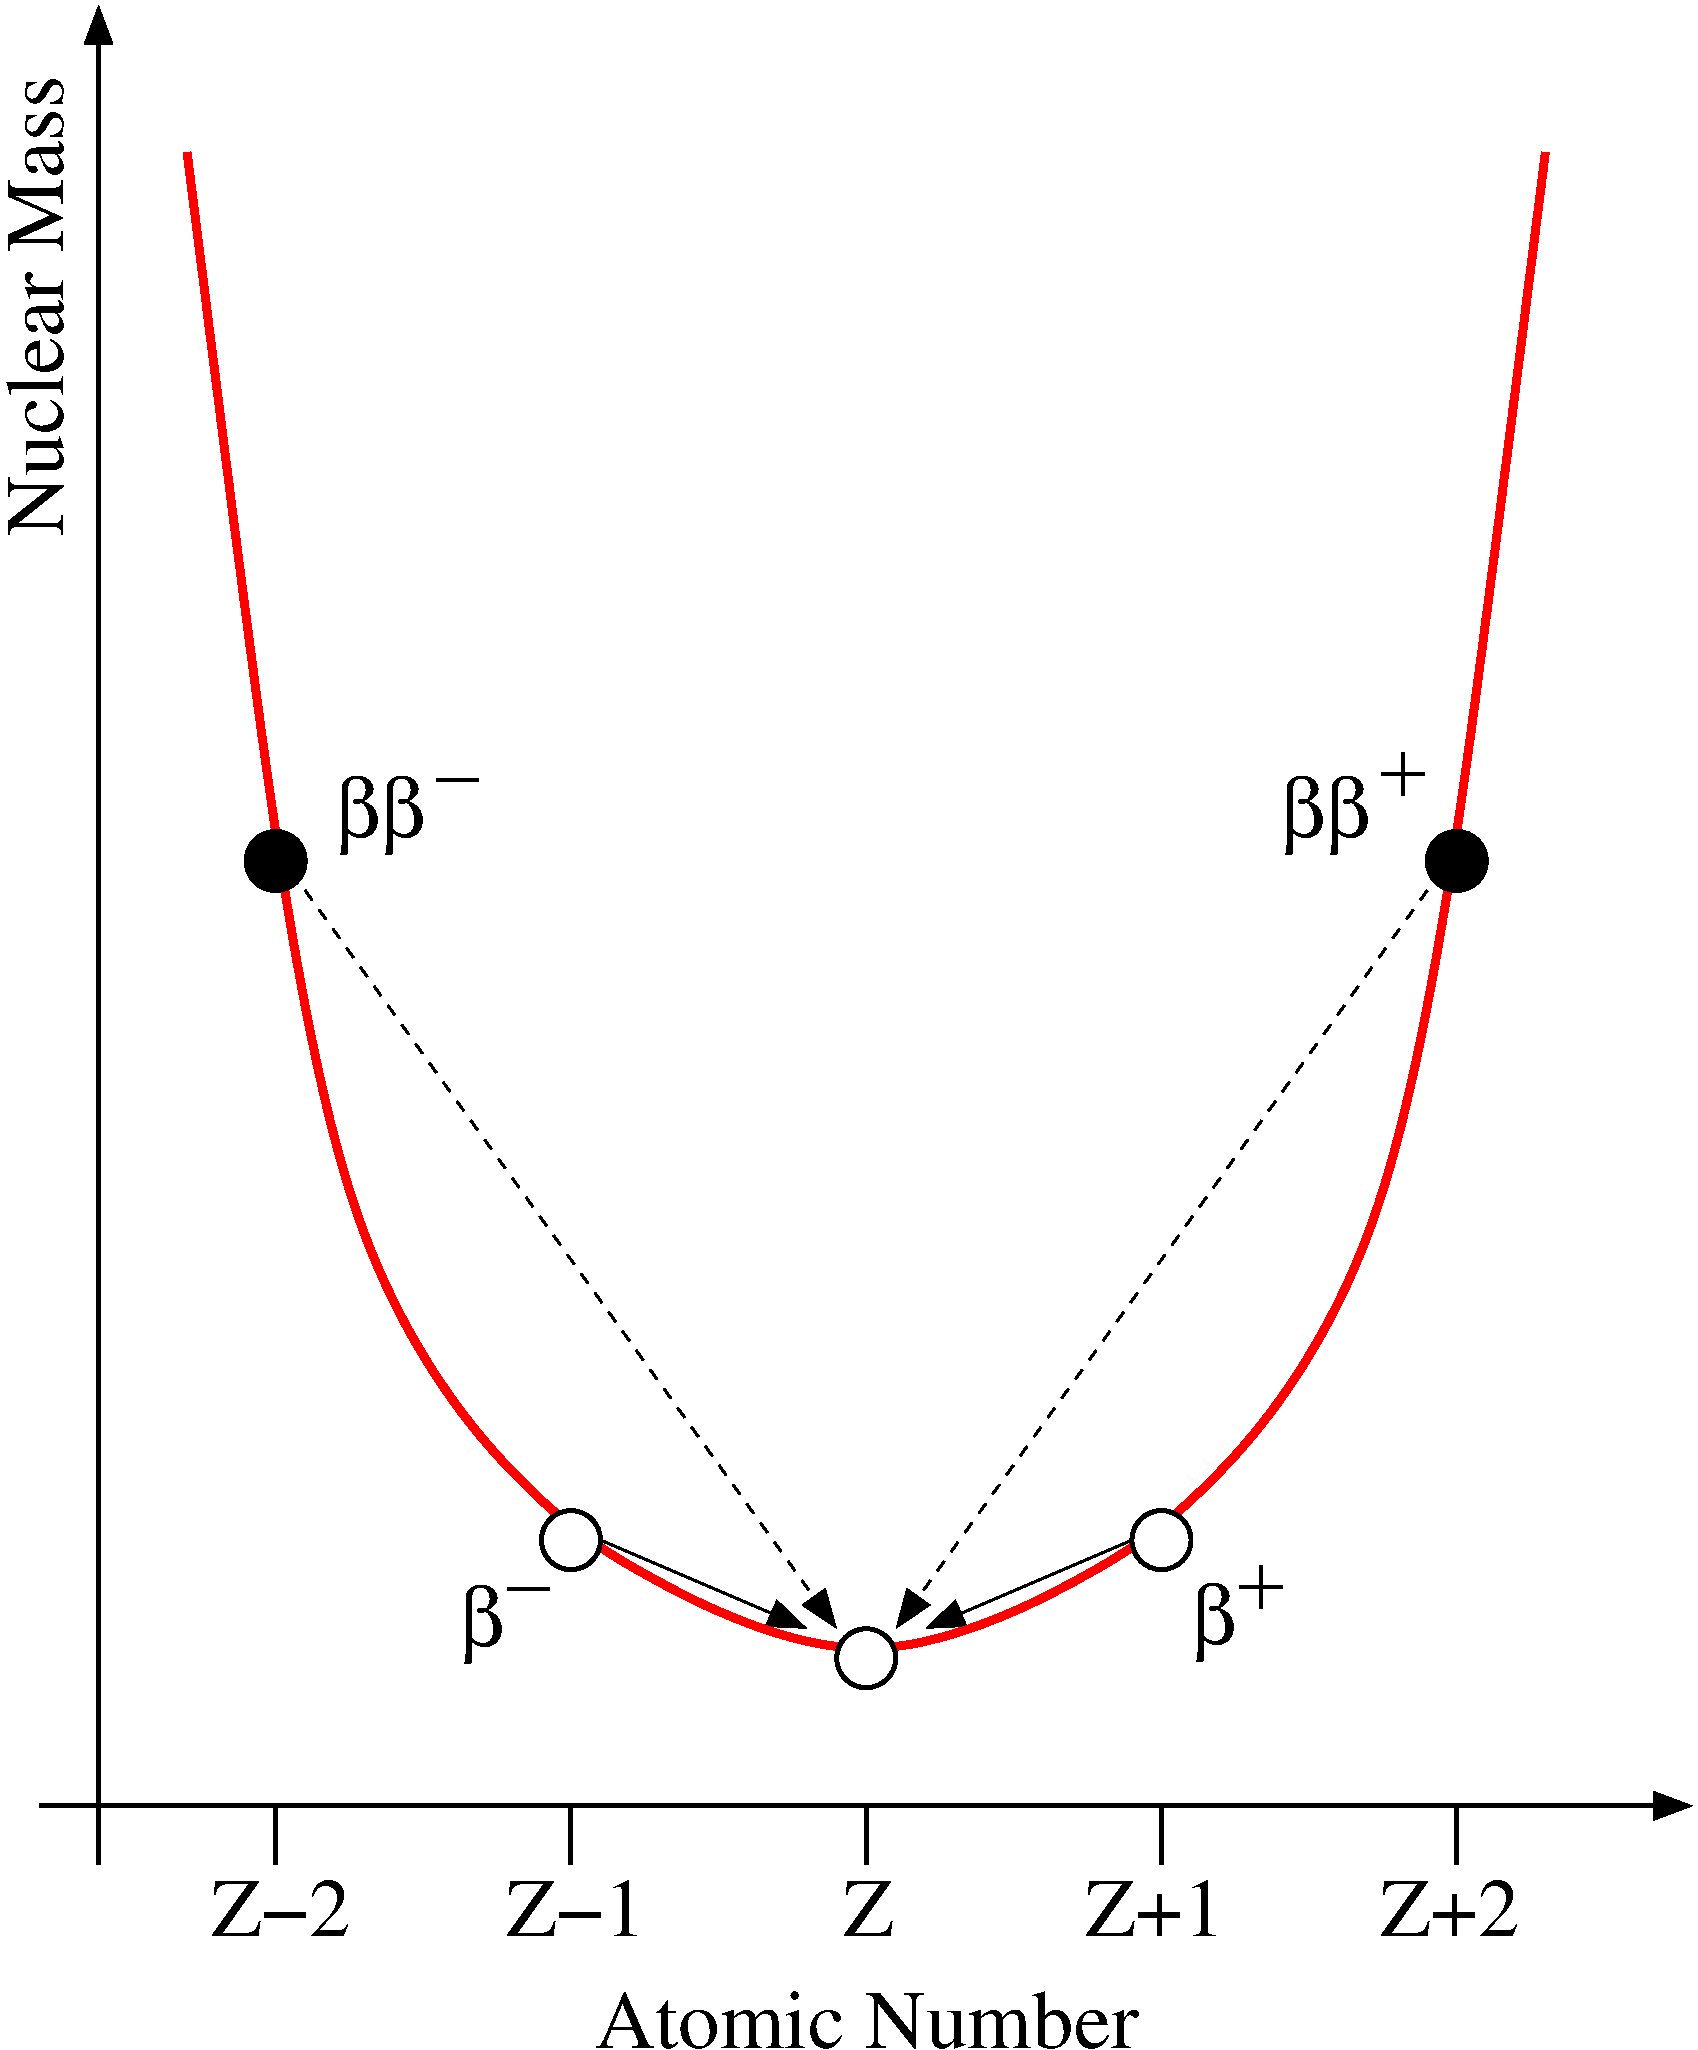
\includegraphics[width=0.9\textwidth]{Figures/parabola_odd_edited.pdf}
\caption[Energy level diagram for odd mass number nuclei.]{Energy level diagram for odd mass number nuclei.}
\label{fig:parabola_odd}
\end{subfigure}
\qqad
\begin{subfigure}[t]{0.45\textwidth}
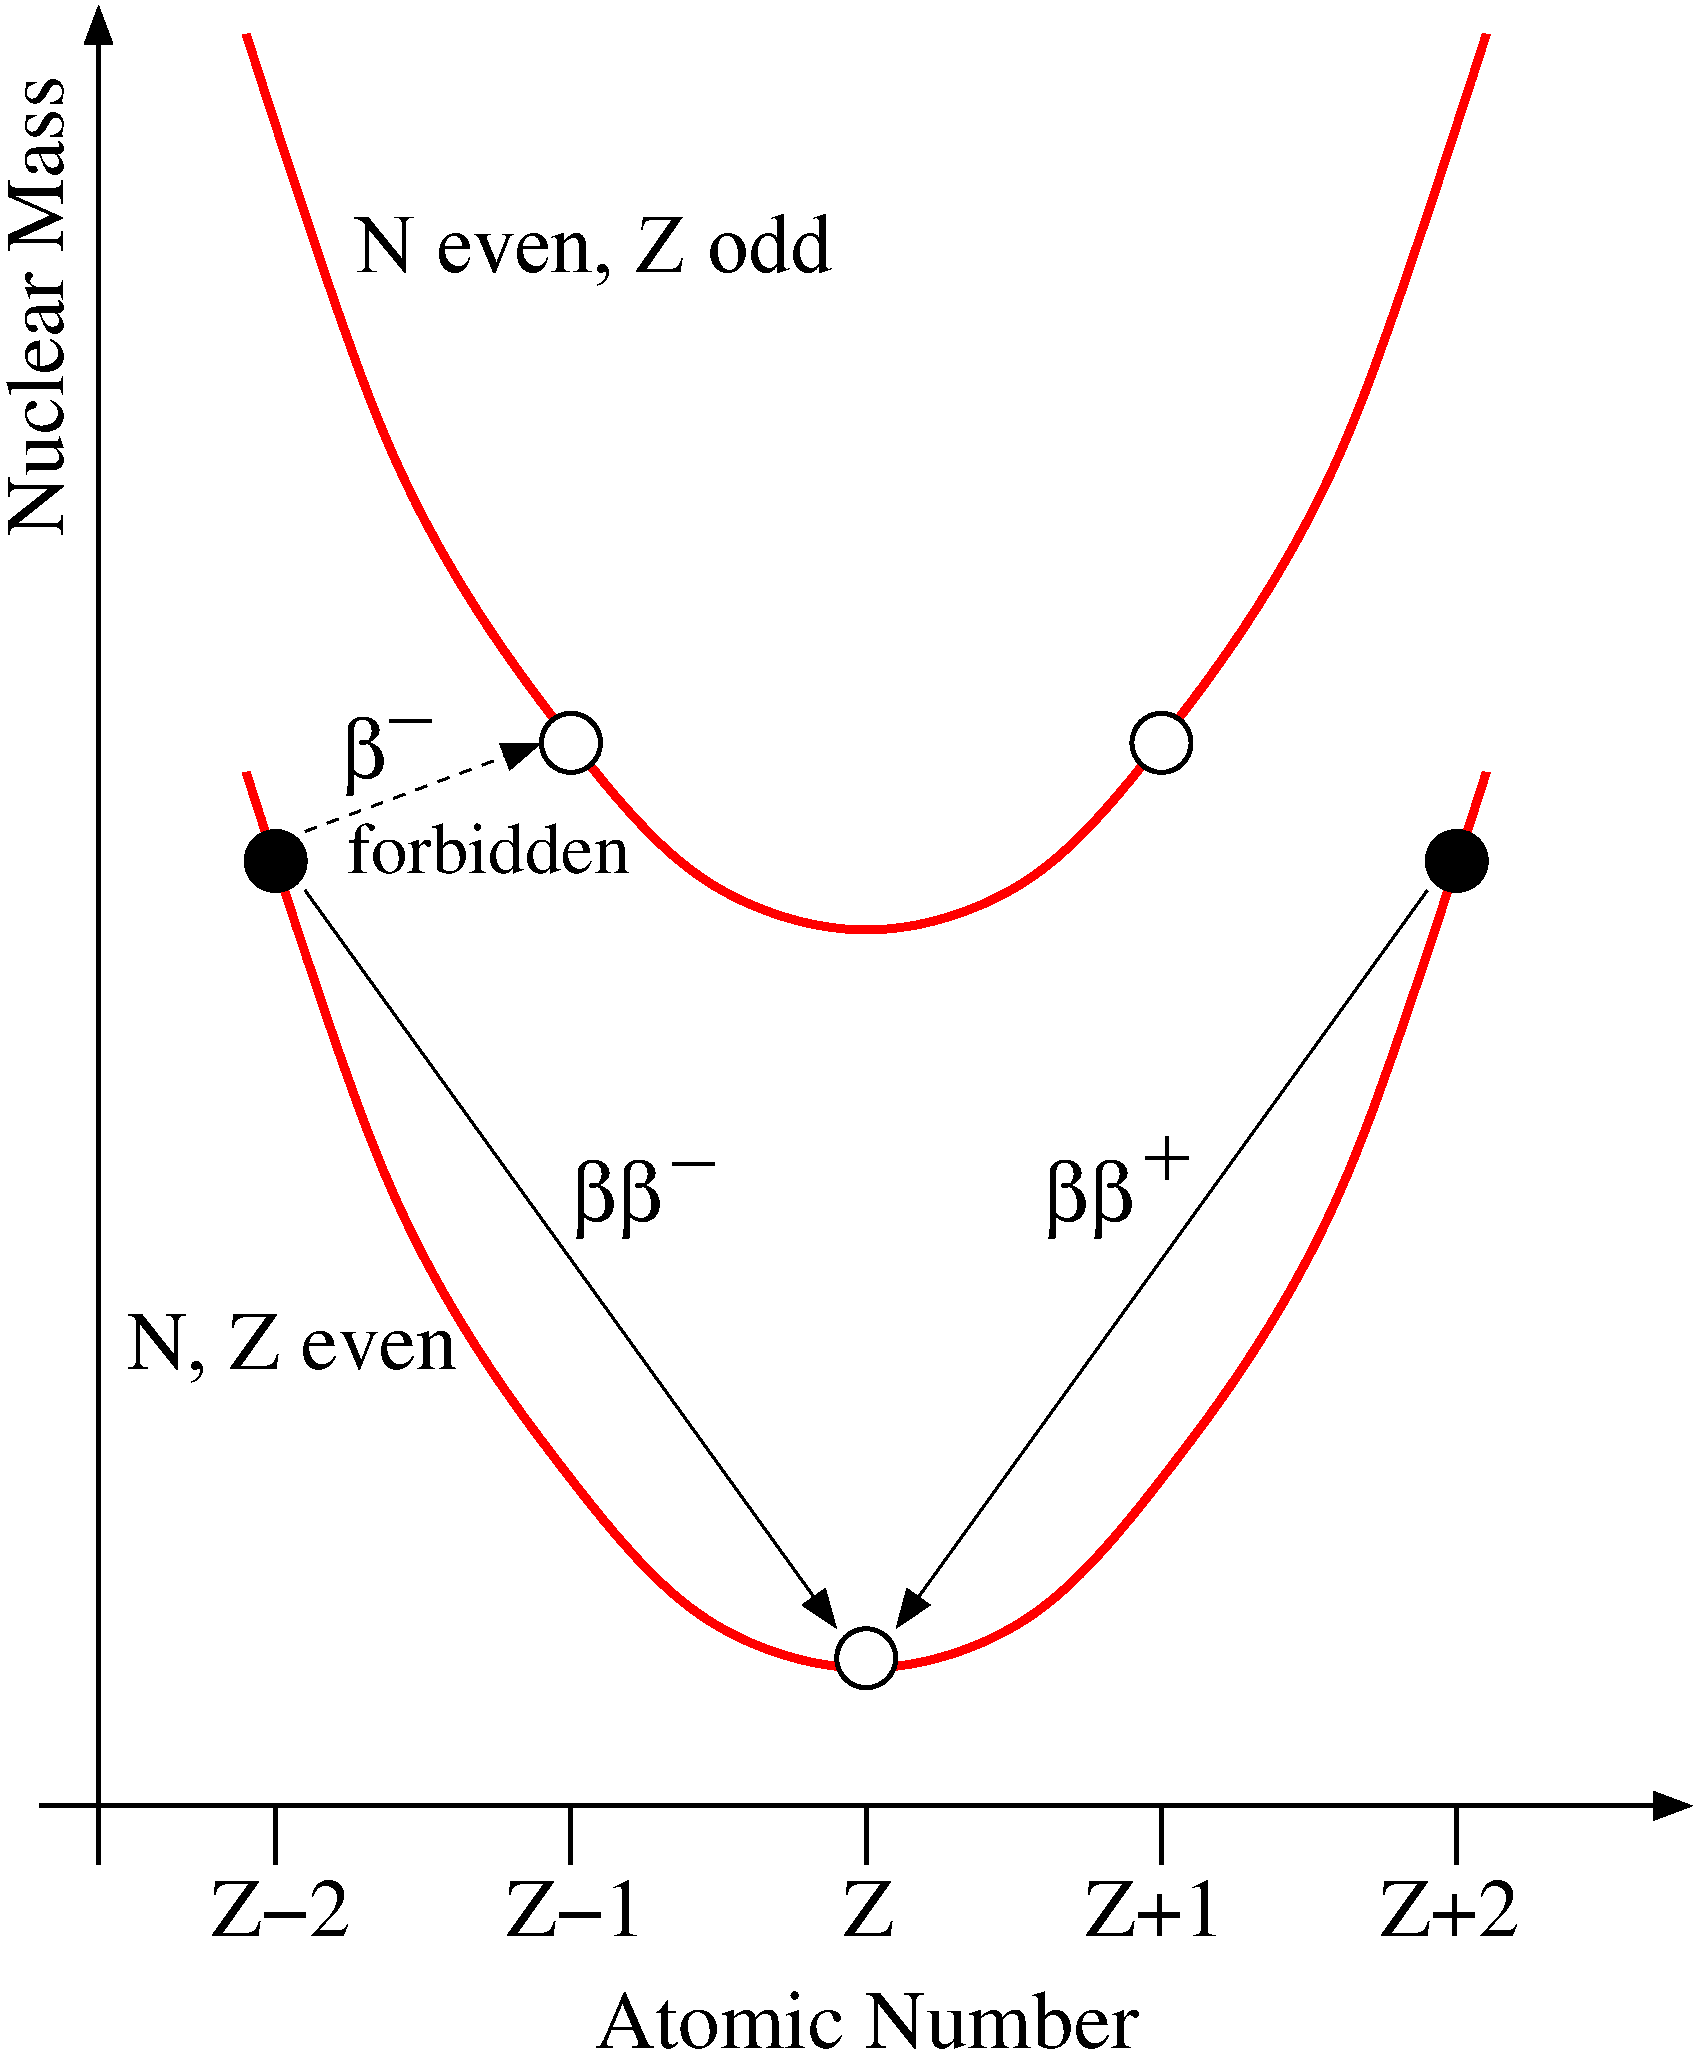
\includegraphics[width=0.9\textwidth]{Figures/parabola_even_edited.pdf}
\caption[[Energy level diagram for even mass number nuclei.]{Energy level diagram for even mass number nuclei.}
\end{subfigure}
\caption[Two sets of double-beta decay candidate nuclei. On the left, an odd mass nucleus allows both single- and double-beta decay, while on the right, an even-even nucleus allows only double-beta decay as single-beta decay is kinematically forbidden.]{Two sets of double-beta decay candidate nuclei. On the left, an odd mass nucleus allows both single- and double-beta decay, while on the right, an even-even nucleus allows only double-beta decay as single-beta decay is kinematically forbidden.}
\label{fig:parabola_even}
\end{figure}

\begin{table}[htpb]
\centering
\begin{tabular}{|c|c|c|}
\hline
Isotope & Half-life, $10^{21}$ years & Experiment \\ \hline 
$^{48}\textrm{Ca}$ & $0.044^{+0.005}_{-0.004} \pm 0.004$ & Nemo-3 \cite{Bongrand:2011ei} \\ \hline
$^{78}\textrm{Ge}$ & $1.926^{+0.025}_{-0.022} \pm 0.092$ & GERDA \cite{Agostini:2015nwa} \\ \hline
$^{82}\textrm{Se}$ & $0.096 \pm 0.003 \pm 0.010$ & NEMO-3 \cite{Bongrand:2011ei}\\ \hline
$^{96}\textrm{Zr}$ & $0.0235 \pm 0.0014 \pm 0.0016$ & NEMO-3 \cite{Bongrand:2011ei}\\ \hline
$^{100}\textrm{Mo}$ & $0.00711 \pm 0.00002 \pm 0.00054$ & NEMO-3 \cite{Bongrand:2011ei}\\ \hline
$^{116}\textrm{Cd}$ & $0.028 \pm 0.001 \pm 0.003$ & NEMO-3 \cite{Bongrand:2011ei} \\ \hline
%^{128}\textrm{Te}$ & $7200 \pm 400$ & Geochemical \\ \hline
$^{130}\textrm{Te}$ & $0.08 \pm 0.02\pm 0.06$ & CUORE-0 \cite{Alduino:2016vtd} \\ \hline
$^{136}\textrm{Xe}$ & $2.165 \pm 0.016 \pm 0.059$ & EXO-200 \cite{Albert:2013gpz} \\ \hline
$^{150}\textrm{Nd}$ & $0.00911^{+0.00025}_{-0.00022}\pm 0.00063$ & NEMO-3 \cite{Bongrand:2011ei} \\ \hline
%$^{238}\textrm{U}$ & $2.0 \pm 0.6$ & Radiochemical \\ \hline
\end{tabular} 
\caption[List of known two-neutrino beta decay half lives.]{List of the known double-beta decay half lives along with the experiment which has the most precise measurement to date. The order of the errors on the half-life are statistical followed by systematic.}
\label{tab:2nuHalfLife}

\begin{comment}
Note for the list of references
\end{comment}

\end{table}

\section{Neutrinoless Double-Beta Decay}
\label{sec:Neutrinoless Double Beta Decay}


\section{State of Neutrinoless Double-Beta Decay Experiments}
\label{sec:State of Neutrinoless Double Beta Decay Experiments}
In addition to CUORE, many other experiments are currently searching and have searched for \zeronubb~ decay. Some of these experiments are listed below and the current status of the field is shown in \autoref{fig:cuore-0-mbetabeta}. As noted before in \autoref{sec:Double Beta Decay} and \autoref{sec:Neutrinoless Double Beta Decay}, the signatures of \zeronubb~ and \twonubb~ decays are a nucleus that interchanges two neutrons and two protons, along with the emission of two electrons and, in the case of \twonubb decay or Majoron emission, two neutrinos and up to two Majorons. Since the half-lives of these decays is so large, (consider that the Universe is only $1.38\times10^{9} yr$ old) an experiment needs to have extremely low background levels in order to be able to even observe these events. As an example, a 1-tonne experiment searching for \zeronubb~decay would expect only $\mathcal{O(10)$ events per year.  This is generally realized in experiments by going to deep underground laboratories to escape cosmic radiation sources and by having pure and clean materials in and near the detector and sources. Also, due to the energies being produced according to a spectrum, all of the backgrounds with energy up to the Q-value will reduce the sensitivity of the measurement. The experiments listed here all seek to identify these signals using a particular technology or set of technologies, some of which, especially in the case of GERDA and MAJORANA, are quite similar to CUORE's. Despite the wide array of technologies, all the experiments below, including CUORE, seek to identify these decays by honing in on and measuring the emitted electron energies as the summed energy spectrum is well-defined as a sharp peak for \zeronubb~or as a broader spectrum for \twonubb~for Majoron emission.

\begin{figure}[htbp]
\centering
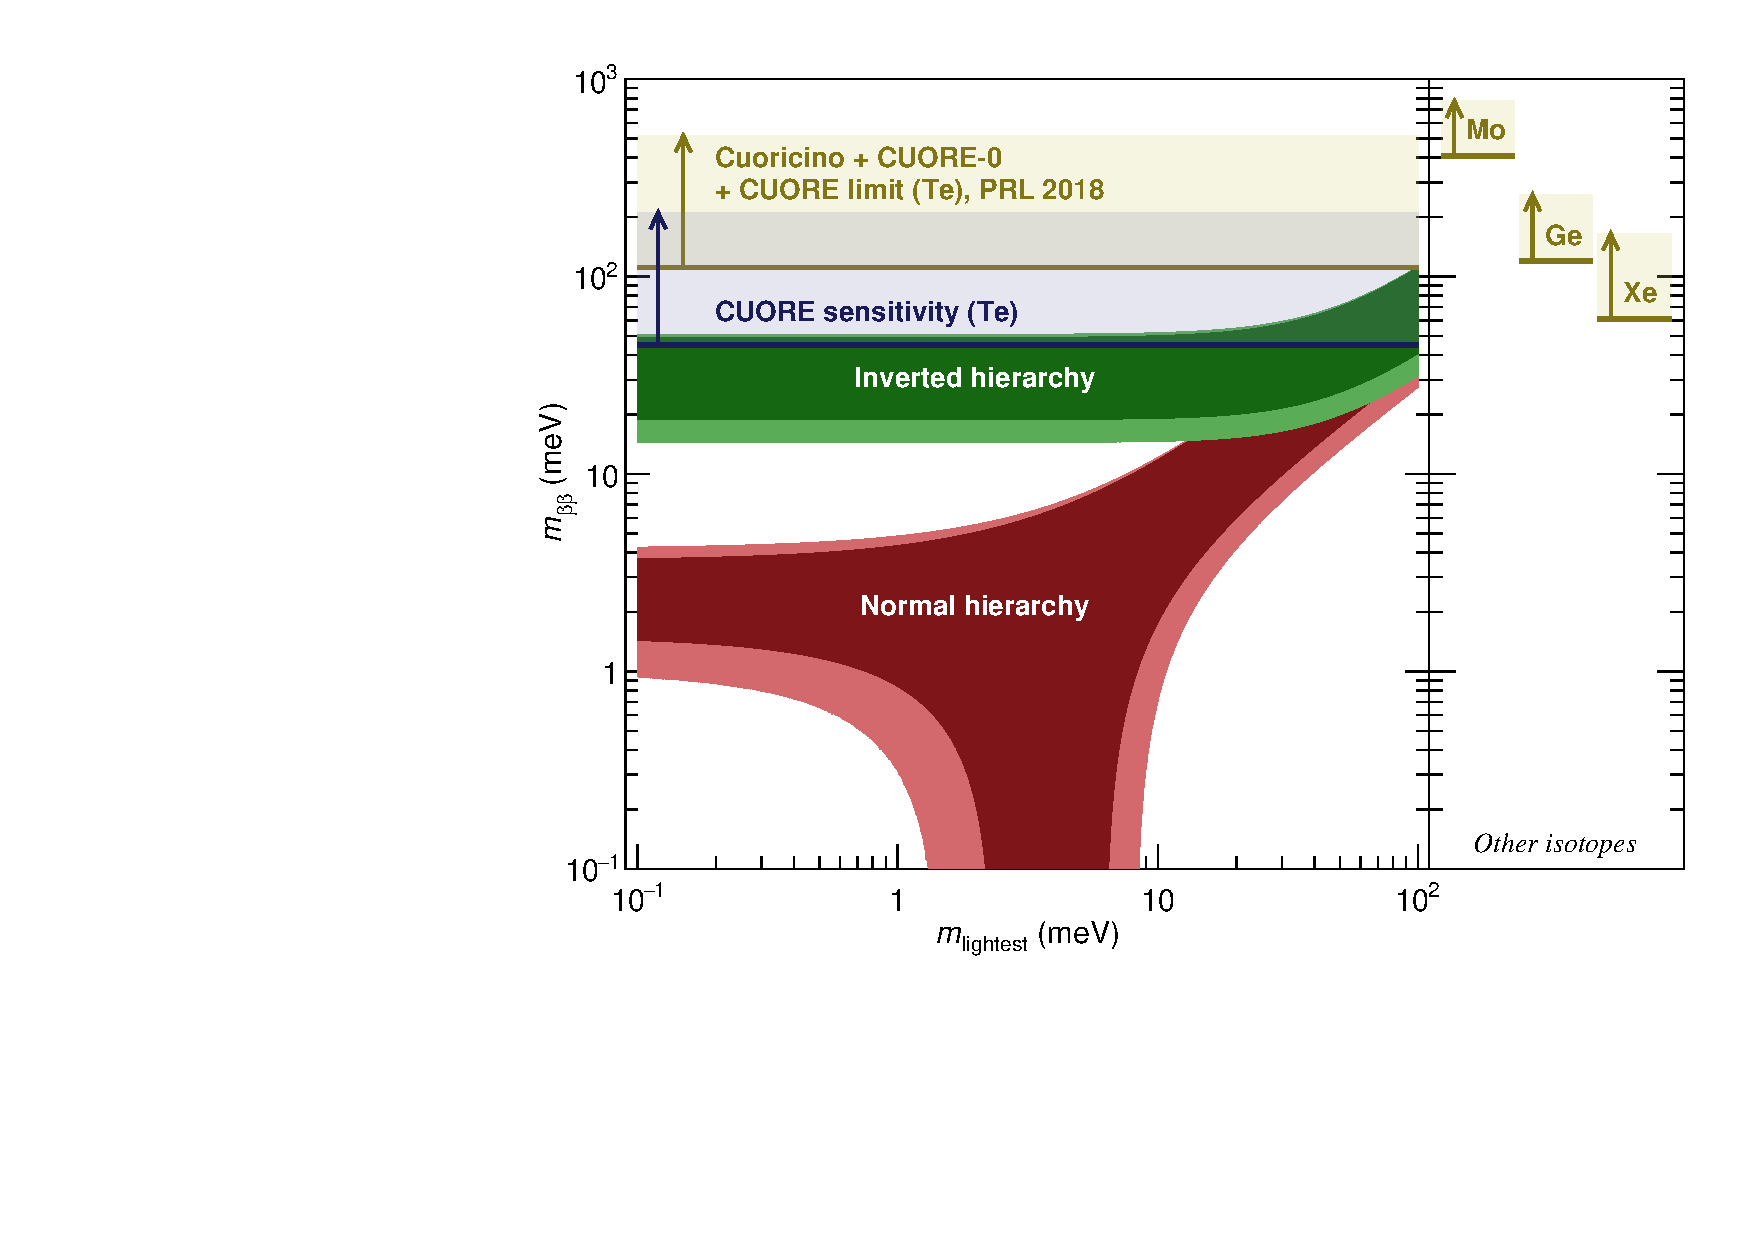
\includegraphics[width=0.7\linewidth]{Figures/M_bb_vs_mlightest_CL_2018.pdf}
\caption{The current status of the field of \zeronubb. The previous experiments in the line of CUORE, CUORE-0 and Cuoricino, have their combined $^{130}$Te result and the results for Mo, Ge, and Xe are shown from NEMO-3, GERDA, and KamLAND-Zen, respectively.}
\label{fig:cuore-0-mbetabeta}
\end{figure}

\subsection{GERDA}

The GERmanium Detector Array (GERDA) Experiment is currently searching for \zeronubb~at the Laboratori Nationali del Gran Sasso (LNGS) using  $^{76}$Ge as the source \cite{Agostini:2017iyd}. Unlike in CUORE, the source is enriched from the natural $7.8\%$ abundance up to $86\%$ and acts acts both the source and the detector of \zeronubb. In the most recent phase of GERDA, Phase II, 37 enriched detectors, 35.6 kg, are assembled along 6 strings around a central string with 3 unenriched detectors. These detectors are then submerged in a 64 $\textrm{m}^3$ LAr cryostat inside a 590 $\textrm{m}^3$ water tank. The water acts as a passive shield for the experiment, while the LAr also acts as an active shield. One of the advantages that CUORE shares with GERDA over other detector technologies is the excellent energy resolution \color{red}[add callback to sensitivity equation]\color{black}. GERDA also takes advantage of the pulse-shape discrimination (PSD) between \zeronubb-like events and $\gamma$-like events in 30 broad energy (BEGe) detectors in addition to scintillation light from the surrounding LAr. With this, the background at $Q_{\beta\beta}$ for the BEGe detectors is low enough at $(0.07^{+1.1}_{-0.5}) \cdot 10^{-3} /(\textrm{keV} \cdot \textrm{kg} \cdot \textrm{yr})$ allowing for the experiment to be considered background-free at the design exposure of $100 \textrm{kg \cdot yr}$. A diagram of the GERDA experimental setup is shown in \autoref{fig:gerda-labelled}.

\begin{figure}[tbph]
\centering
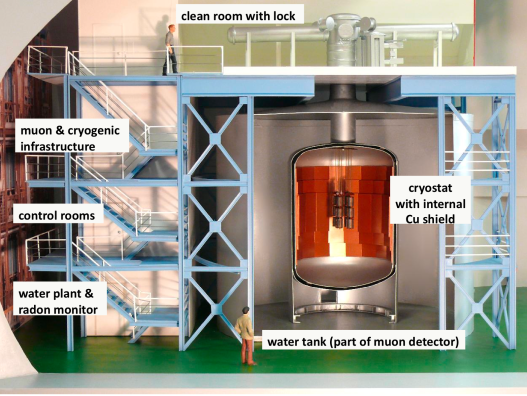
\includegraphics[width=0.7\linewidth]{Figures/gerda-view.png}
\caption{Diagram of the GERDA detector. Liquid argon is also inside the copper shielding with the detectors submerged.}
\label{fig:gerda-labelled}
\end{figure}

\subsection{MAJORANA}

\subsection{KamLAND-Zen}
The Kamioka Liquid Scintillator Antineutrino Detector Zero neutrino double beta decay search (KamLAND-Zen) searches for \zeronubb~in 90.8\% enriched $^{136}$Xe \cite{KamLAND-Zen:2016pfg}. This experiment uses the existing infrastructure from the KamLAND experiment, which acted as a  The detector uses the Xe as a liquid scintillator acting as both the source and detector of \zeronubb. Xe benefits from self-shielding due to the attenuation length of gammas in xenon which allows for reduced levels of background in the innermost volume. This is a distinct advantage over experiments such as CUORE, MAJORANA, and GERDA, as their detectors need to be held in place and cannot self-shield as a result. However, the energy resolution of the KamLAND-Zen is significantly worse than the $\mathcal{O}(\textrm{keV})$ resolution in these experiments. A diagram of the KamLAND-Zen detector is shown in \autoref{fig:kamlandzen}}.

\begin{figure}[tbph]
\centering
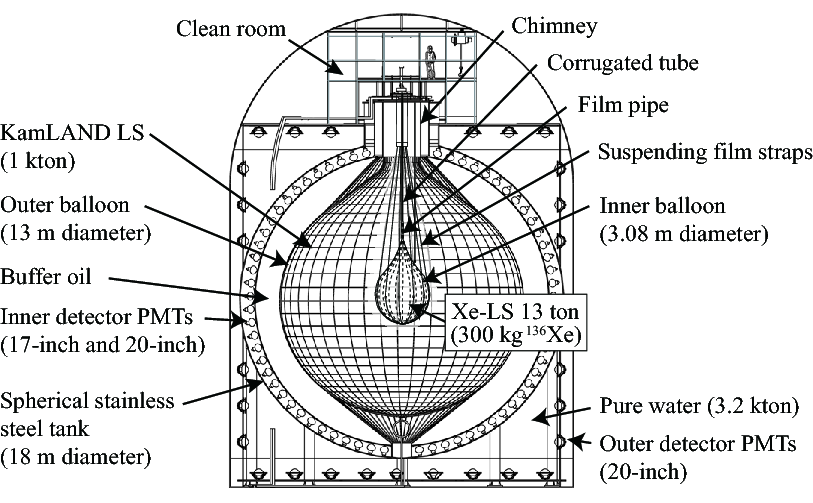
\includegraphics[width=0.7\linewidth]{Figures/KamlandZen}
\caption{A schematic of the Kamland-Zen experimental apparatus. The Xe-loaded liquid scintillator is held within the balloon at the center. Figure from \cite{::2015uaa}.}
\label{fig:kamlandzen}
\end{figure}

\subsection{EXO}

\subsection{NEMO-3}
The Neutrino Ettore Majorana Observatory (NEMO-3) collected \twonubb~data from multiple isotopes including $^{100}$Mo, $^{82}$Se, $^{130}$Te, $^{116}$Cd, $^{150}$Nd, $^{96}$Zr, and $^{48}$Ca \cite{Bongrand:2011ei}. NEMO-3 also searched for \zeronubb~in $^{100}$Mo, $^{82}$Se, $^{48}$Ca, and $^{150}$Nd \cite{Bongrand:2011ei}\cite{::2016dpe}\cite{Arnold:2016ezh}. Unlike the other experiments listed in this section, NEMO-3 did not utilize a ``detector = source" method, instead using separate detectors and sources. An advantage of this method is that the two emitted electrons can be tracked and measured separately, which is a clear signal that a decay occured as a vertex can be reconstructed along with the energies. An example track in NEMO-3 is shown in \autoref{fig:nemo3393042373top2}. Another advantage is that the source foil can be easily replaced with other isotopes while leaving the rest of the detector apparatus unchanged. However, this is a constraint on the size of the source, as it needs to be small enough for electrons to traverse and be detected outside, yet the number of decays scales with the source mass.

\begin{figure}[htbp]
\centering
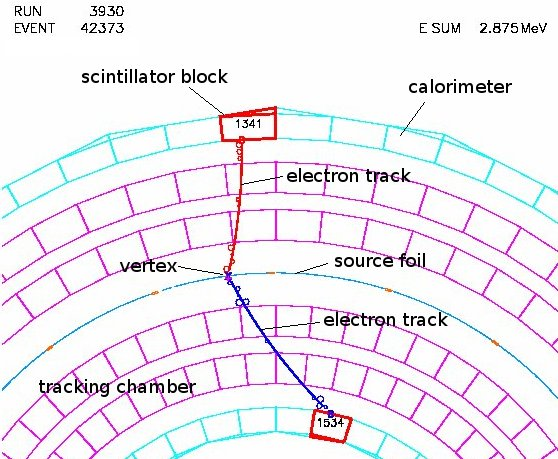
\includegraphics[width=0.7\linewidth]{Figures/nemo3_3930_42373_top_2}
\caption{A \zeronubb~candidate event from NEMO-3. The electrons are emitted from a nucleus in the source foil and deposit energy in the calorimeter after leaving tracks in the tracking chamber.}
\label{fig:nemo3393042373top2}
\end{figure}


\begin{comment}


In the laboratory, the fundamental interactions shown in \hyperref[fig:0nuBB]{Fig. \ref*{fig:0nuBB}} and \hyperref[fig:2nuBB]{Fig. \ref*{fig:2nuBB}} are measured as decays of specific nuclei. In particular, double beta decay occurs when two neutrons or two protons in a nucleus spontaneously decay, typically from the ground state of the initial nucleus (A,~Z) to the ground state of the final nucleus (A,~Z$\pm$2). By energy conservation, the change in energy from the initial to the final nucleus, called the Q-value, is given in roughly equal amounts to the final state particles: the two electrons, and, in the case of \twonubb, the two neutrinos. The nuclear recoil is negligible in these decays as the nuclei involved are much more massive than the electrons and the neutrinos. 

When detecting double beta decay, the neutrinos pass undetected through the detector volume and only the electrons can be measured. Thus, the energies reconstructed by the electrons will be a continuous spectrum up to the Q-value for \twonubb~and a single peak at the Q-value for \zeronubb~\hyperref[fig:2nubbspectrum]{Fig. \ref*{fig:2nubbspectrum}}.

\begin{figure} [h]
\centering
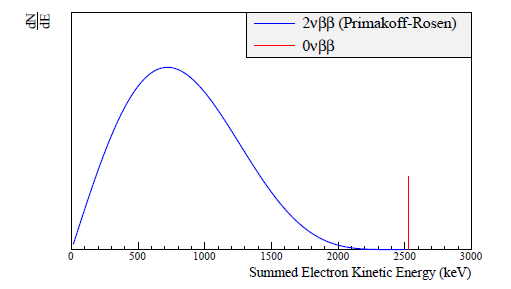
\includegraphics[width=0.7\linewidth]{Figures/2nuBBSpectrum.png}
\caption{An example spectrum for double beta decay. The amplitude of the \zeronubb~decay is not shown to scale.}
\label{fig:2nubbspectrum}
\end{figure}


\subsection{\twonubb}
In general, it is difficult to measure double beta decay as it is a second-order weak process. The exception to this occurs in some even-even nuclei wherein single beta decay is energetically forbidden, but double beta decay is allowed. Of the 35 naturally occurring isotopes where double beta decay is possible, 12 of them have been measured in the laboratory. Of particular importance for this work is the double beta decay half-life for $^{130}\textrm{Te}$ at $7.0 \pm 0.9 \pm 1.1 \times 10^{20}~\textrm{years}$ as measured by the NEMO-3 collaboration \cite{Arnold:2011gq}. As the longest measured alpha decay is $^{209}\textrm{Bi}$ with a half-life of $1.9 \times 10^{19}~\textrm{years}$ \cite{Marcillac:2003Bi-209detection}, double-beta decay half lives are the longest nuclear decays that have been measured.

Since the half-life is so large, an experiment needs to have low background levels in order to be able to observe these events. This is generally realized in experiments by going to deep underground laboratories to escape cosmic radiation sources and by having pure and clean materials in and near the detector and sources. Also, due to the energies being produced according to a spectrum, all of the backgrounds with energy up to the Q-value will reduce the sensitivity of the measurement.

\begin{center}
\begin{tabular}{|c|c|c|}
\hline 
Isotope & Half-life, $10^{21}$ years & Experiment \\ \hline 
$^{48}\textrm{Ca}$ & $0.044^{+0.005}_{-0.004} \pm 0.004$ & Nemo-3 \\ \hline
$^{78}\textrm{Ge}$ & $1.84^{+0.09~+0.11}_{-0.08~-0.06}$ & GERDA (2013) \\ \hline
$^{82}\textrm{Se}$ & $0.096 \pm 0.003 \pm 0.010$ & NEMO-3 \\ \hline
$^{96}\textrm{Zr}$ & $0.0235 \pm 0.0014 \pm 0.0016$ & NEMO-3 \\ \hline
$^{100}\textrm{Mo}$ & $0.00711 \pm 0.00002 \pm 0.00054$ & NEMO-3 \\ \hline
$^{116}\textrm{Cd}$ & $0.028 \pm 0.001 \pm 0.003$ & NEMO-3 \\ \hline
%^{128}\textrm{Te}$ & $7200 \pm 400$ & Geochemical \\ \hline
$^{130}\textrm{Te}$ & $0.7 \pm 0.09\pm 0.11$ & NEMO-3 \\ \hline
$^{136}\textrm{Xe}$ & $2.165 \pm 0.016 \pm 0.059$ & EXO-200 \\ \hline
$^{150}\textrm{Nd}$ & $0.00911^{+0.00025}_{-0.00022}\pm 0.00063$ & NEMO-3 \\ \hline
%$^{238}\textrm{U}$ & $2.0 \pm 0.6$ & Radiochemical \\ \hline
\end{tabular} 
\end{center}
\end{comment}
